\documentclass{article}
\usepackage[utf8]{inputenc}
\usepackage{graphicx}

\title{SVM}
\author{Ramya HOUNTONDJI}
\date{Décembre 2020}

\begin{document}

\maketitle

\section{Introduction}

Connaissez-vous l’apprentissage automatique, ou machine learning en anglais? Concrètement, il s’agit d’une branche de l’informatique, qui englobe les algorithmes qui apprennent par eux-mêmes. Celà veut dire qu'initialement, un algorithme d’apprentissage automatique ne sait rien faire; puis, au fur et à mesure qu’il s’entraîne sur des données, il est capable de répondre de plus en plus efficacement à la tâche qu’on lui demande de faire. 

\vspace{5mm} %5mm vertical space
Nous pouvons classer les algorithme en deux catégories:
\vspace{5mm} %5mm vertical space
  -les algorithmes classiques, où l’algorithme se contente d’appliquer une série de règles sans apprendre des cas précédents.
  -les algorithmes d’apprentissage automatique, où l’algorithme est capable d’effectuer un apprentissage à partir des données déjà vues.
\vspace{5mm} %5mm vertical space
Dans ce document nous allons parler de la deuxième catégorie dalgorithme et plus précisement des SMV.
Sans plus tarder commençons!
\vspace{5mm} %5mm vertical space
\section{Généralités sur les SVM}
\vspace{5mm} %5mm vertical space

Une machine à vecteurs de support, traduction littérale pour Support Vector Machine, est un algorithme d’apprentissage automatique supervisé qui peut être utilisé à des fins de classification et de régression. Les SVM sont plus généralement utilisés dans les situations de classification.
Ils ont été développés dans les années 1990.  
Leur principe est simple : il ont pour but de séparer les données en classes à l’aide d’une frontière aussi « simple » que possible, de telle façon que la distance entre les différents groupes de données et la frontière qui les sépare soit maximale.
Cette distance est aussi appelée « marge » et les SVMs sont ainsi qualifiés de « séparateurs à vaste marge », les « vecteurs de support » étant les données les plus proches de la frontière.

\begin{figure}[b!]
  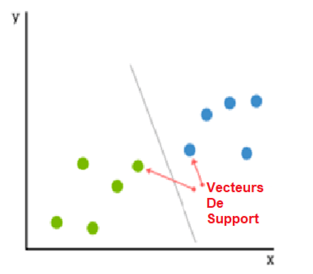
\includegraphics[width=\linewidth]{1.PNG}
  \caption{Généralités.}
  \label{fig1:SVM}
\end{figure}
\vspace{5mm} %5mm vertical space
Avant toute chose, nous allons commencer par éclaircir le terme Classification.
Considérons l’exemple ci dessus. On se place dans le plan, et l’on dispose de deux catégories: les ronds rouges et les carrés bleus, chacune occupant une région différente du plan.
Cependant, la frontière entre ces deux régions n’est pas connue. 
Ce que l’on veut, c’est que quand on lui présentera un nouveau point dont on ne connaît que la position dans le plan, l’algorithme de classification sera capable de prédire si ce nouveau point est un carré rouge ou un rond bleu.

Notre problème de classification se traduit dont comme suit: pour chaque nouvelle entrée, être capable de déterminer à quelle catégorie cette entrée appartient.
Autrement dit, il faut être capable de trouver la frontière entre les différentes catégories.
Si on connaît la frontière, savoir de quel côté de la frontière appartient le point, et donc à quelle catégorie il appartient.

\vspace{5mm} %5mm vertical space
\begin{figure}[b!]
  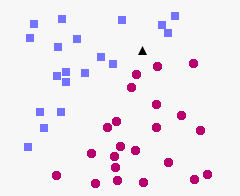
\includegraphics[width=\linewidth]{classification 1.PNG}
  \caption{algorithme de classification}
  \label{fig2:algorithme de classification}
\end{figure}
\vspace{5mm} %5mm vertical space
Le SVM est une solution à ce problème de classification1.
Il appartient à la catégorie des classificateurs linéaires (qui utilisent une séparation linéaire des données), et qui dispose de sa méthode à lui pour trouver la frontière entre les catégories.

Pour que le SVM puisse trouver cette frontière, il est nécessaire de lui donner des données d’entraînement. En l’occurrence, on donne au SVM un ensemble de points, dont on sait déjà si ce sont des carrés rouges ou des ronds bleus, comme dans la figure précédente. A partir de ces données, le SVM va estimer l’emplacement le plus plausible de la frontière: c’est la période d'entraînement, nécessaire à tout algorithme d’apprentissage automatique.

Une fois la phase d’entraînement terminée, le SVM a ainsi trouvé, à partir de données d’entraînement, l’emplacement supposé de la frontière. 
En quelque sorte, il a «appris» l’emplacement de la frontière grâce aux données d’entraînement. 
De plus, il est maintenant capable de prédire à quelle catégorie appartient une entrée qu’il n’avait jamais vue avant, et sans intervention humaine.
\vspace{5mm} %5mm vertical space
\begin{figure}[b!]
  \includegraphics[width=\linewidth]{choix frontière.PNG}
  \caption{choix de la frontière}
  \label{fig2}
\end{figure}
\vspace{5mm} %5mm vertical space
Comme vous pouvez le constater dans la figure ci-dessous, le SVM a choisi une ligne droite comme frontière. 
C’est parce que, comme dit plus haut, le SVM est un classificateur linéaire. 
Bien sûr, la frontière trouvée n’est pas la seule solution possible, et n’est probablement pas optimale non plus.

Cependant, il est considéré que, étant donné un ensemble de données d’entraînement, les SVM sont des outils qui obtiennent parmi les meilleurs résultats.
En fait, il a même été prouvé que dans la catégorie des classificateurs linéaires, les SVM sont ceux qui obtiennent les meilleurs résultats.

Un des autres avantages des SVM, et qu’il est important de noter, est que ces derniers sont très efficaces quand on ne dispose que de peu de données d’entraînement: alors que d’autres algorithmes n’arriveraient pas à généraliser correctement, on observe que les SVM sont beaucoup plus efficaces. 
Cependant, quand les données sont trop nombreuses, le SVM a tendance à baisser en performance.

Le but du  SVM, est donc  d’apprendre à bien placer la frontière entre deux catégories. 

\vspace{5mm} %5mm vertical space
\begin{figure}[b!]
  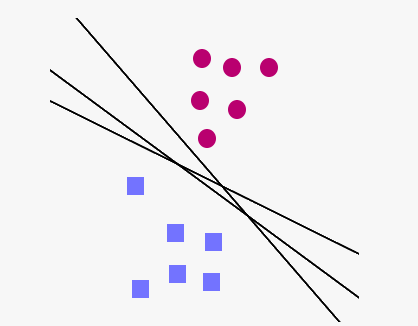
\includegraphics[width=\linewidth]{choix_h.PNG}
  \caption{choix de la frontière}
  \label{fig3:}
\end{figure}
\vspace{5mm} %5mm vertical space

\vspace{5mm} %5mm vertical space
Maintenant que l'objectif de cet algorithme est cerné, nous pouvons aller plus en détail.
\vspace{5mm} %5mm vertical space
\section{Explications, étapes  et aspects mathématiques}

\vspace{5mm} %5mm vertical space
\subsection{Formalisme sur les SVM}
\vspace{5mm} %5mm vertical space
De façon plus générale que dans l'exemple donné précédemment, les SVM ne se bornent pas à séparer des points dans le plan. 
Ils peuvent en fait séparer des points dans un espace de dimension quelconque.
Par exemple, si on cherche à classer des fleurs par espèce, alors que l’on connaît leur taille, leur nombre de pétales et le diamètre de leur tige, on travaillera en dimension 3.

Un autre exemple est celui de la reconnaissance d’image: une image en noir et blanc de 28*28 pixels contient 784 pixels, et est donc un objet de dimension 784. Il est ainsi courant de travailler dans des espaces de plusieurs milliers de dimensions.

Fondamentalement, un SVM cherchera simplement à trouver un hyperplan qui sépare les deux catégories d'un problème.

\vspace{5mm} %5mm vertical space
\subsection{Les hyperplans}
\vspace{5mm} %5mm vertical space
\textbf{Précisions sur les hyperplans}
\vspace{5mm} %5mm vertical space
Dans un espace vectoriel de dimension finie $n$, un hyperplan est un sous-espace vectoriel de dimension $n-1$. Ainsi, dans un espace de dimension $2$ un hyperplan sera une droite, dans un espace de dimension $3$ un hyperplan sera un plan, etc.

Soit un espace vectoriel $E$ de dimension $n$. L’équation caractéristique d’un hyperplan est de la forme $w_1 x_1+w_2 x_2+\dots+w_n x_n=0$, où $w_1, \dotsc, w_n$ sont des scalaires. Par définition, tout vecteur $x = \left( \begin{array}{c} x_1 \\ \vdots \\ x_n \end{array} \right) \in E$ vérifiant l’équation appartient à l’hyperplan. Par exemple, en dimension $2$, $ax+by=0$ est bien l’équation caractéristique d’une droite vectorielle (qui passe par l’origine).

De plus, un hyperplan sépare complètement l’espace vectoriel en deux parties distinctes. Ainsi, une ligne droite sépare le plan en deux régions distinctes; et en dimension $3$, c’est le plan qui joue le rôle de ce séparateur: il y a un demi-espace «d’un côté» du plan, et un autre demi-espace «de l’autre côté» du plan. Avec un hyperplan, il est donc possible de diviser notre espace vectoriel en deux catégories distinctes: tout pile ce qu’il nous faut pour notre problème de classification!
\vspace{5mm} %5mm vertical space
Comme vous pouvez le constater, un hyperplan vectoriel passe toujours par $0$. C’est pour cette raison qu’on utilisera un \textbf{hyperplan affine}, qui n’a pas quant à lui obligation de passer par l’origine.



Ainsi, si l’on se place dans $\mathbb{R}^n$, pendant son entraînement le SVM calculera un hyperplan vectoriel d’équation $w_1 \cdot x_1 + w_2\cdot x_2+ \dots +w_n\cdot x_n=0$, ainsi qu’un scalaire (un nombre réel) $b$. C’est ce scalaire $b$ qui va nous permettre de travailler avec un hyperplan affine, comme nous allons le voir.



Le vecteur $w= \left( \begin{array}{c} w_1 \\ \vdots \\ w_n \end{array} \right)$ est appelé \textbf{vecteur de poids}, le scalaire $b$ est appelé \textbf{biais}.



Une fois l’entraînement terminé, pour classer une nouvelle entrée $x=\left( \begin{array}{c} a_1 \\ \vdots \\ a_n \end{array} \right) \in \mathbb{R}^n$, le SVM regardera le signe de:



$$h(x)= w_1 a_1 + \dots + w_n a_n + b = \sum_{i=1}^n w_i \cdot a_i+b = w^\top \cdot x+b$$



Si $h(x)$ est positif ou nul, alors $x$ est d’un côté de l’hyperplan affine et appartient à la première catégorie, sinon $x$ est de l’autre côté de l’hyperplan, et donc appartient à la seconde catégorie.



En résumé, on souhaite savoir, pour un point $x$, s’il se trouve d’un côté ou de l’autre de l’hyperplan. La fonction $h$ nous permet de répondre à cette question, grâce à la classification suivante:



\[ \begin{cases}
h(x) \geq 0  \implies x \in \text{catégorie 1} \\
h(x) < 0 \implies x \in \text{catégorie 2}
\end{cases} \]

\vspace{5mm} %5mm vertical space
\subsection{Entrainement des svm}
\vspace{5mm} %5mm vertical space
Ainsi, étant donnés un hyperplan de vecteur de poids $w$, et de biais $b$, nous pouvons calculer si un point $x_k$ appartient à telle ou telle catégorie, grâce au signe de $h(x_k)$.



En particulier, supposons que l’on assigne à tout point $x_k$ un label $l_k$ qui vaut $1$ si $x_k$ appartient à la première catégorie, et $-1$ si $x_k$ appartient à la seconde catégorie. Alors, si le SVM est correctement entraîné, on a toujours $l_k h(x_k) \geq 0$, c’est-à-dire $l_k (w^\top \cdot x_k+b)\geq0$. \\
Le but d’un SVM, lors de l’entraînement, est donc de trouver un vecteur de poids $w$ et un biais $b$ tels que, pour tout $x_k$ de label $l_k$ appartenant aux données d’entraînement, $l_k (w^\top \cdot x_k+b)\geq 0$. Autrement dit, de trouver un hyperplan séparateur entre les deux catégories.
\vspace{5mm} %5mm vertical space
\begin{figure}[b!]
  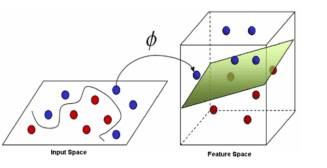
\includegraphics[width=\linewidth]{hyperplan2.PNG}
  \caption{Hyperplan.}
  \label{fig5:SVM}
\end{figure}
\vspace{5mm} %5mm vertical space

Comme on l’a vu précédemment, on choisira l’hyplerplan qui maximise la marge, c’est-à-dire la distance minimale entre les vecteurs d’entraînement et l’hyperplan. De tels vecteurs situés à la distance minimale sont appelés vecteurs supports.
\vspace{5mm} %5mm vertical space
C’est de là que vient le nom des SVM. En effet, on peut prouver que l’hyperplan donné par un SVM ne dépend que des vecteurs supports, c’est donc tout naturellement qu’on a appelé cette structure les Support Vectors Machines, c’est-à-dire les machines à vecteur support.
\vspace{5mm} %5mm vertical space
\subsection{Calculs de marges}
\vspace{5mm} %5mm vertical space
Si l’on prend un point $x_k \in \mathbb{R}^n$, on peut prouver que sa distance à l’hyperplan de vecteur support $w$ et de biais $b$ est donnée par\textsuperscript{\ref{footnote:3}} :
$$\frac{l_k (w^\top \cdot x_k+b)}{\|w\|}$$



où $\|w\|$ désigne la norme euclidienne de $w$. La marge d’un hyperplan de paramètres $(w,b)$ par rapport à un ensemble de points $(x_k)$ est donc $\min\limits_k  \frac{l_k (w^\top \cdot x_k+b)}{\|w\|}$. Pour rappel, la marge est la distance minimale de l’hyperplan à un des points d’entraînement.
\vspace{5mm} %5mm vertical space
\subsection{Maximisation de la marge}
\vspace{5mm} %5mm vertical space
On veut trouver l’hyperplan de support $w$ et de biais $b$ qui permettent de maximiser cette marge, c’est-à-dire qu’on veut trouver un hyperplan avec la plus grande marge possible. Cela permettra, intuitivement, d’être tolérant face aux petites variations. \\
Cette intuition est justifiée : en 1995, le Russe Vladimir Vapnik a prouvé que cette maximisation produit un hyperplan optimal, c’est-à-dire qui donnera lieu au moins d’erreurs possible (on parle de \textit{capacité de généralisation maximale}).
\vspace{5mm} %5mm vertical space
\begin{figure}[b!]
    \centering
    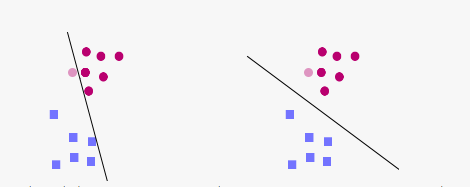
\includegraphics{généralisation.PNG}
    \caption{Généralisation pour maximiser la marge}
    \label{fig7:my_label}
\end{figure}
 
\vspace{5mm} %5mm vertical space
Puisque l’on cherche l’hyperplan qui maximise la marge, on cherche l’unique hyperplan dont les paramètres $(w, b)$ sont donnés par la formule : $\displaystyle \mathop{\operatorname{arg\,max}}\limits_{w,\,b}\min\limits_k \frac{l_k (w^\top \cdot x_k+b)}{\|w\|}$ .
\vspace{5mm} %5mm vertical space
\subsection{Normalisation et résolution du problème}
\vspace{5mm} %5mm vertical space
Même si on peut montrer que l’hyperplan optimal est unique, il existe plusieurs couples $(w, b)$ qui décrivent ce même hyperplan\textsuperscript{\ref{footnote:4}}. On décide de ne considérer que l’unique paramétrage $(w, b)$ tel que les vecteurs support $x_s$ vérifient $l_s (w^\top \cdot x_s + b) = 1$. Par conséquent, $\forall k, \, l_k (w^\top \cdot x_k+b)\geq1$, et l’égalité est atteinte si $x_k$ est un vecteur support. Dit autrement, cette normalisation sur $w$ et $b$ permet de garantir que la marge $\min\limits_k \frac{l_k (w^\top \cdot x_k+b)}{\|w\|}$ est alors de \$ \textbackslash{}frac 1\{|w|\}\$.



Le problème d’optimisation de la marge $\displaystyle\mathop{\operatorname{arg\,max}}\limits_{w,\,b}\min\limits_k \frac{l_k (w^\top \cdot x_k+b)}{\|w\|}$ se simplifie ainsi en $\displaystyle\mathop{\operatorname{arg\,max}}\limits_{w,\,b} \frac{1}{\|w\|}$, tout en gardant en tête nos hypothèses de normalisation, à savoir $\forall k, \, l_k (w^\top \cdot x_k+b) \geq 1$.



On se retrouve donc avec le problème suivant :
$\begin{cases}
\text{maximiser} \quad \frac{1}{\|w\|}\\ 
\text{sous les contraintes}\quad \forall k, \, l_k (w^\top \cdot x_k+b)\geq 1
\end{cases}$



Que l’on peut reformuler de la façon suivante :
$\begin{cases}
\text{minimiser} \quad\|w\|\\ 
\text{sous les contraintes}\quad \forall k, \, l_k (w^\top \cdot x_k+b)\geq 1
\end{cases}$



Que, pour des raisons pratiques, on reformule à nouveau :
$\begin{cases}
\text{minimiser} \quad\frac{\|w\|^2}{2}\\ 
\text{sous les contraintes}\quad \forall k, \, l_k (w^\top \cdot x_k+b)\geq 1
\end{cases}$



Ce genre de problème est appelé \textbf{problème d’optimisation quadratique}, et il existe de nombreuses méthodes pour le résoudre. Dans le cas présent, on utilise la méthode des multiplicateurs de Lagrange, que le lecteur intéressé pourra consulter sur \externalLink{ce PDF}{http://www.engr.mun.ca/\textasciitilde{}baxter/Publications/LagrangeForSVMs.pdf} (en anglais).



Cette résolution donnera une valeur optimale pour $w$, mais rien pour $b$. Pour retrouver $b$, il suffit de se rappeler que pour les vecteurs support, $l_s (w^ \top \cdot x_s+b)=1$. On en déduit donc que $b$ est tel que $\min\limits_k\, l_k (w^\top \cdot x_k  +b) =1$.
\vspace{5mm} %5mm vertical space
le SVM est à présent entraîné, et nous pouvons l’utiliser pour classer des données qu’il n’avait jusqu’à présent jamais vues (en utilisant notre fonction de classification h)
\vspace{5mm} %5mm vertical space
\section{Utilisations , limites et moyens d'implémentation}
\vspace{5mm} %5mm vertical space
\subsection{Utilisations et limites}
\vspace{5mm} %5mm vertical space
Les SVM sont utilisés pour les problèmes de classification de texte telles que l’attribution de catégorie, la détection du spam ou encore l’analyse des sentiments.
Ils sont également couramment utilisés pour les problèmes de reconnaissance d’image, particulièrement en reconnaissance de forme et en classification de couleur. Il joue  un rôle essentiel dans de nombreux domaines de la reconnaissance manuscrite des symboles, tels que les services d’automatisation postale.
\vspace{5mm} %5mm vertical space
 Aussi, leS SVM sont utilisés dans une variété d’applications (bioinformatique, recherche d’informations, vision par ordinateur, finance, etc.) notamment parce qu’à la différence des réseaux de neurones, on peut les utiliser sans comprendre leur fonctionnement.
\vspace{5mm} %5mm vertical space
On peut également s'en servir pour:
\begin{itemize}
\item\relax Classer des fleurs suivant leur espèce, en fonction de la longueur et largeur de leurs pétales et sépales.
\item\relax En médecine, les SVM sont utilisés pour reconnaître, par la diffusion dans le cerveau d’altérations liées aux AVC.
\item\relax \externalLink{Pour la reconnaissance de caractères sur des plaques d’immatriculation
\item\relax En médecine encore, pour l'identification des gènes responsables de certains types de cancer.
\end{itemize}
\vspace{5mm} %5mm vertical space
En terme d'inconvénient, on peut noter: qu'ils ne  conviennent pas aux jeux de données plus volumineux, car le temps d’entraînement avec les SVM peut être long et qu'ils sont moins efficaces sur les jeux de données contenant du bruits et beaucoup d’outliers.
\vspace{5mm} %5mm vertical space

\subsection{Moyens d'implémentation}
\vspace{5mm} %5mm vertical space
Si vous  souhaitez travailler sur les svm, vous pouvez utiliser des bibliothèques.

\vspace{5mm} %5mm vertical space
\begin{itemize}
\item\relax En  Python 3, vous pouvez vous servir de \textbf{scikit}, plus précisément de sklearn.svm.
\item\relax En Java, vous pouvez utiliser LIBSVM, qui a également été portée en Matlab, Python, Ruby, Perl, NodeJS, bindée en PHP…
\end{itemize}
\vspace{5mm} %5mm vertical space
\section{CONCLUSION}

Nous arrivons à la fin de ce document. En espérant que les informations qui ont été apportées vous seront utiles, je vous souhaite un bon apprentissage.
\vspace{5mm} %5mm vertical space

\end{document}
